\documentclass[10pt]{beamer}

\usetheme{metropolis}
\usepackage{appendixnumberbeamer}

\usepackage{booktabs}
\usepackage[scale=2]{ccicons}

\usepackage{pgfplots}
\usepgfplotslibrary{dateplot}

\usepackage{xspace}
\newcommand{\themename}{\textbf{\textsc{metropolis}}\xspace}

\usepackage[spanish]{babel}

\usepackage{graphicx}

% Paquetes necesarios
\usepackage[dvipsnames]{xcolor}
\usepackage{amsmath}
\usepackage{listings}
\usepackage{color}


% Configuración de listings para código fuente
\lstdefinelanguage{JavaScript}
{
  keywords = {typeof, new, true, false, function, return, null, switch, var, if, in, while, do, else, case, break, class, export, boolean, throw, implements, import, this, constructor, string, number, public, private, static, const, var, let, void},
  morekeywords = [2]{class, export, boolean, throw, implements, import, this, interface},
  morekeywords = [3]{Promise, Observable},
  morekeywords = [4]{log},
  otherkeywords = {;},
  comment = [l]{//},
  morecomment = [s]{/*}{*/},
  morestring = [b]',
  morestring = [b]",
}

\lstset
{
  language= JavaScript,
  commentstyle = {\color{OliveGreen}},
  stringstyle = {\color{green}},
  keywordstyle = {\color{orange}\bfseries},
  keywordstyle = [2]{\color{orange}},
  keywordstyle = [3]{\color{purple}},
  keywordstyle = [4]{\color{lime}},
  keywordstyle = [5]{\color{orange}},
  basicstyle = {\ttfamily \color{main-color}},
  backgroundcolor = {\color{back-color}},    
  sensitive = false,
  breaklines = true,
  showstringspaces= false,
  showspaces= false,
  extendedchars= true
}


\title{React}
\subtitle{Una biblioteca en Javascript para crear interfaces}
\date{\today}
\author{Betology}
\institute{Amor, comprensión y ternura}
% \titlegraphic{\hfill\includegraphics[height=1.5cm]{logo.pdf}}

\begin{document}

\maketitle

\begin{frame}{Table of contents}
  \setbeamertemplate{section in toc}[sections numbered]
  \tableofcontents[hideallsubsections]
\end{frame}

% Sección 1: ¿Qué es React?
\section{¿Qué es React?}

\begin{frame}

  \begin{itemize}
    \item Biblioteca de JavaScript para construir interfaces de usuario.
    \item Desarrollada por Facebook.
    \item Utiliza componentes para construir interfaces modulares y reutilizables.
  \end{itemize}
\end{frame}

% Sección 2: Componentes de React
\section{Componentes de React}

% Diapositiva 1: Definición de un Componente
\begin{frame}[fragile]
  \frametitle{Definición de un Componente}
  \begin{itemize}
    \item Los componentes son bloques de construcción en React.
    \item Pueden ser definidos como clases o funciones.
  \end{itemize}
    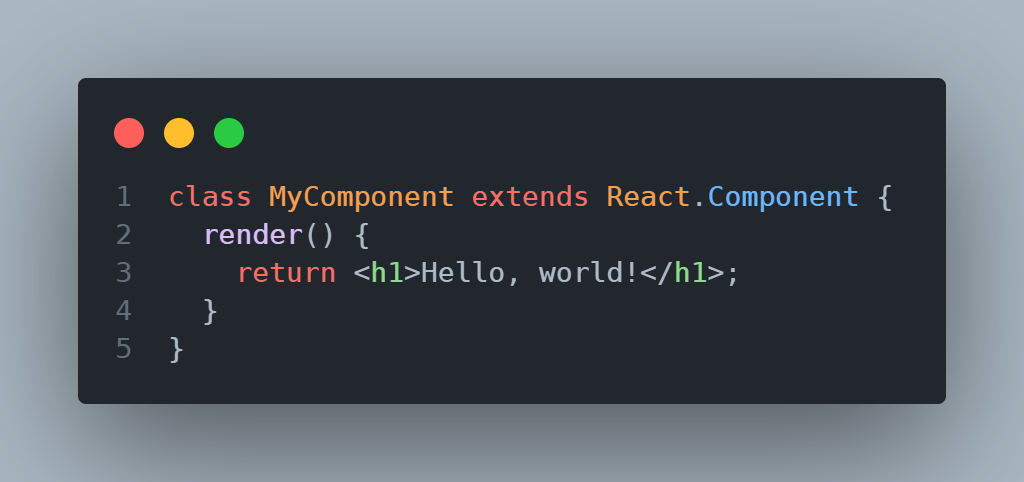
\includegraphics[width=100mm,scale=0.25]{myComponent.png}
\end{frame}

% Diapositiva 2: Componentes Funcionales
\begin{frame}[fragile]
  \frametitle{Componentes Funcionales}
  \begin{itemize}
    \item Más simples y fáciles de escribir.
    \item No tienen estado propio (antes de los Hooks).
  \end{itemize}
    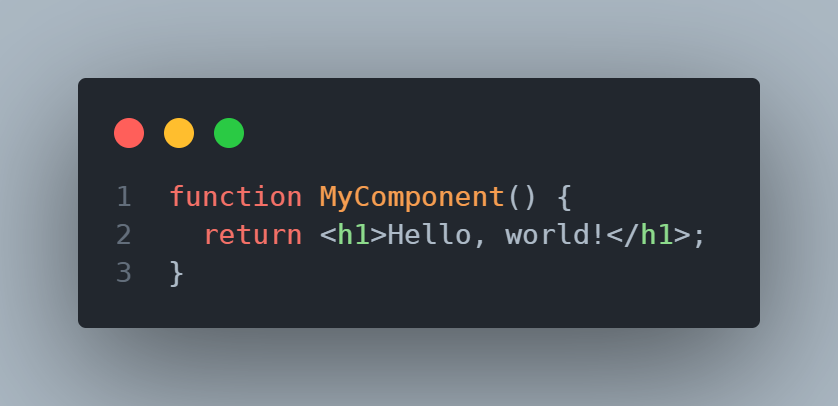
\includegraphics[width=75mm,scale=0.25]{myComponentFunction.png}
\end{frame}


\end{document}
